\section{Wetter-API(Datenquelle)}
In diesem Kapitel wird auf die im Rahmen dieses Projektes Wetter-API vom Anbieter "Openweathermap" und die anschließend eigens dafür implementierte Schnittstelle zu dieser. Anschließend werden die für die Schnittstelle  implementierten Test beschrieben. Abschließend wird diese Komponente gegen die zu beginn Definierten Anforderungen validiert. 
\subsection{Die API}
Der Anbieter "OpenWeatherMap" bietet kostenlos die Möglichkeit Wetterdaten via http-Request abzufragen. 
Hierzu ist lediglich ein Nutzerzugang erforderlich, welchen sich jeder anlegen kann. Es können verschiedene Vorhersagen abgefragt werden, für diese Arbeit beschränkt es sich jedoch auf die tägliche Vorhersage und eine  5-tages Vorhersage. Solch ein angesprochener Http-Request (hier für eine 5tägige Vorhersage) setzt sich wie folgt zusammen, 
\begin{lstlisting}
http://api.openweathermap.org/data/2.5/forecast?zip=78467,de&
APPID=41c464d95d33fabc24d44a5086ea9848
\end{lstlisting}

Der Parameter "ZIP" wird zum setzten der Postleitzahl für die gewünschte Stadt genutzt, zu diesem muss noch das Länderkürzel hinzugefügt werden. Die "APPID" wird von "OpenweatherMap" für jeden Nutzeraccount spezifisch vergeben und dient als Authentifizierung. Der Parameter"forecast" dient zur Unterscheidung zwischen einer aktuellen Vorhersage und einer 5-tages Vorhersage, bei Erster würde der Request wie folgt aussehen, 

\begin{lstlisting}
http://api.openweathermap.org/data/2.5/weather?zip=78467,de&
APPID=41c464d95d33fabc24d44a5086ea9848
\end{lstlisting}

hier muss lediglich der Parameter "forecast" durch "weather" ersetzt werden. 

"OpenWeatherMap" unterscheidet das Angebot zwischen kostenfrei und kostenpflichtig. Innerhalb der kostenpflichtigen Varianten gibt es Staffelungen, das gesamte Angebot wird aus Abb. \ref{img:OpenWeather} genauer ersichtlich. 

Für die in dieser Arbeit beschriebenen Lösung wurde auf die kostenfreie Variante gesetzt. Daher musste bei der Implementierung auf einige Einschränkungen geachtet werden, zu diesen gehören, 

\begin{itemize}
\item "Calls per minute (no more than)",
\item "Availibilty",
\item "Weather API data update".
\end{itemize}

Da auf das kostenfreie Modell gebaut wird, muss vor allem auf die erstgenannte Einschränkung (Abb. \ref{img:OpenWeather}) geachtet werden. Laut dieser sind lediglich 60 Requests mit den oben gezeigten URLs erlaubt. Im Rahmen der gesamten Anwendung wurde entscheiden, dass diese Applikation für alle Hauptstädte der 16 Bundesländer und Konstanz zur Verfügung stehen soll. Somit errechnet sich der Anteil an Requests pro Minute wie folgt,

\begin{align}
RequestsPerMin. = (16*2)+(2*2)\\
RequestsPerMin. = 36
\end{align}
somit kann ohne auf Probleme zu stoßen, ein Request-Intervall von 60 Sekunden, gewählt werden. 

\begin{figure}[!ht]
	\centering
	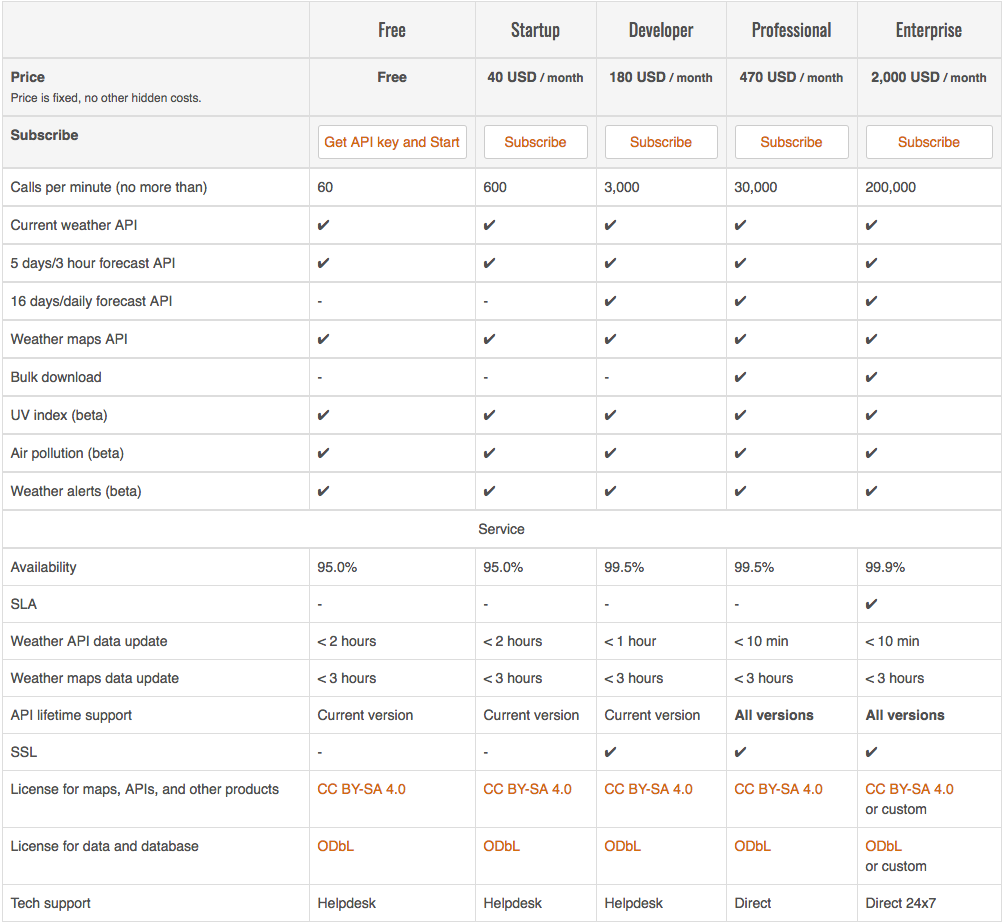
\includegraphics[width=1.0\textwidth]{Bilder/OpenWeatherMap.png}
	\caption{OpenWeatherMap Konditionen}
	\label{img:OpenWeather}
\end{figure} 
Im Bezug auf den "Response-Type" der API, kann entschieden werden, ob als "Response-Type" das Json- oder XML-Format gewählt werden soll. Aufgrund der guten Möglichkeiten von Java mit Json-Dokumente zu arbeiten, wurde  das Json-Format, als "Response-Type", gewählt.
Um bessere Vorstellungen von solch einem Response im Json-Format zu bekommen wird dieser untenstehend am Beispiel einer täglichen Vorhersage gezeigt.  

  \begin{lstlisting}
{"coord":{"lon":9.16,"lat":47.67},"weather":[{"id":800,"main":"Clear","description":"clear sky","icon":"01d"}],"base":"stations","main":{"temp":297.6,"pressure":1021,"humidity":41,"temp_min":296.15,"temp_max":298.15},"visibility":10000,"wind":{"speed":5.7,"deg":30},"clouds":{"all":0},"dt":1497797400,"sys":{"type":1,"id":4915,"message":0.0038,"country":"DE","sunrise":1497756293,"sunset":1497813872},"id":0,"name":"Konstanz","cod":200}
\end{lstlisting}

Des weiteren wird am nächsten Beispiel der Response-Type für die 5-tägige Vorhersage aufgezeigt, jedoch wird hier aufgrund des hohen Umfangs nur ein kleiner Teil (für 3 Stunden) gezeigt. Im Normalfall besteht ein vollständiger Response aus im 3 stunden Takt 
folgenden Informationen für 5 Tage.
 
  \begin{lstlisting}
{"cod":"200","message":0.0035,"cnt":40,"list":[{"dt":1497808800,"main":{"temp":295.56,"temp_min":294.226,"temp_max":295.56,"pressure":957.98,"sea_level":1034.02,"grnd_level":957.98,"humidity":53,"temp_kf":1.34},"weather":[{"id":800,"main":"Clear","description":"clear sky","icon":"01d"}],"clouds":{"all":0},"wind":{"speed":2.46,"deg":51.5021},"sys":{"pod":"d"},"dt_txt":"2017-06-18 18:00:00"}
\end{lstlisting}
\clearpage
Um mit diesen Json-Response-Types besser und freier arbeiten zu können wurde eine Schnittstelle implementiert, welche die Daten vorher Filtert, somit werden nur wichtige Informationen genutzt. Die Implementierung dieser Schnittstelle wird im folgenden Abschnitt beschrieben. Die Schnittstelle greift die Grundlagen und Problemstellungen der "OpenWeatherMap" -API auf, welche in diesem Abschnitt beschrieben wurden, von den Request-Intervallen bis hin zu den zwei verschiedenen Arten von Vorhersagen.

\subsection{Die Schnittstelle}
\subsection{Die Komponenten}
\subsection{Testing}
\subsection{Anforderungen}
\begin{table}[!ht]
  \centering
    \begin{minipage}{15cm}
      \centering
      \begin{tabular}{*{3}{|l|p{5.0cm}|p{5.0cm}}}\hline
      \multicolumn{4}{|c|}{\cellcolor[RGB]{200,200,200}Validierung nach "12 Faktor APP"} \\\hline
     \textbf{ID}&\textbf{Anforderung}&\textbf{Validierungs Element}&\textbf{Erfüllt}\\\hline
     1.&Codebase&....&Nein\\
      \hline
     2.&Abhängigkeiten&....&Nein\\
     \hline
     3.&Konfiguration&....&Nein\\
     \hline
     4.&Unterstützende Dienste&....&Nein\\
     \hline 
     5.&Build, release, run&....&Nein\\
     \hline
     6.&Prozesse&....&Nein\\
     \hline
      7.&Bindung an Ports&....&Nein\\
     \hline
      8.&Nebenläufigkeit&....&Nein\\
     \hline
      9.&Einweggebrauch&....&Nein\\
     \hline
     10.&Dev-Prod-Vergleichbarkeit&....&Nein\\
     \hline     
     11.&Logs&....&Nein\\
     \hline
     12.&Admin-Prozesse&....&Nein\\
     \hline
      \end{tabular}
   \caption{Validierung nach "12 Faktor APP"}\label{tab:Anforderungen}
    \end{minipage}
\end{table}

ToDo: Verweis auf 12 Faktor APP Standard !!! 